\section{Domain walls in curved ferromagnetic wires}\label{sec:domain_walls}

The purpose of this section is to describe curvature-induced effects in statics and dynamics of the one-dimensional topological soliton -- domain wall (DW). Here we will consider DWs in \textit{parabola}- and \textit{Euler spiral} shaped wires, see Figs.~\ref{fig:Geometries_n_curvatures}(d) and \ref{fig:Geometries_n_curvatures}(e), respectively.

Only transversal DWs will be considered in this section.

Within this section, for the further analysis it is convenient to rewrite the total micromagnetic energy~\eqref{eq:total_energy} by using the angular parameterization $\vec{m} = \cos\Theta \, \vec{e}_{\textsc{t}}+\sin\Theta \,\left(\cos\Phi \, \vec{e}_{\textsc{n}} + \sin \Phi \, \vec{e}_{\textsc{b}}\right)$, where $\Theta=\Theta(\overline{t},\xi)$ and $\Phi=\Phi(\overline{t},\xi)$ are magnetic angles. With this angular notations, one can rewrite the total micromagnetic energy~\eqref{eq:total_energy}  as
\begin{equation}\label{eq:dw_total_energy_angular}
\begin{split}
\mathcal{E} =  \, \int\limits^{+ \infty}_{-\infty}\mathrm{d}\xi \, \bigl[(\Theta' + \varkappa \, \cos \Phi)^2 +& (\Phi' \, \sin \Theta  - \varkappa \, \cos \Theta \, \sin \Phi)^2\\
&- \cos^2 \Theta + \varepsilon \sin^2\Theta\sin^2\Phi\bigr].
\end{split}
\end{equation}
In \eqref{eq:dw_total_energy_angular} it is taken into account that a plane wires have zero torsion. Here, $\varepsilon = K_p / K<1$ is an anisotropy ratio\footnote{It is known that the magnetostatic energy of a straight and uniformly magnetized stripe with rectangular cross section can be reduced to the effective shape anisotropy~\cite{Aharoni98}. This approximation also valid for curved ribbons/stripes~\cite{Gaididei19}.}.

\subsection{Statics of the domain wall.}

The equilibrium magnetization states correspond to the minimum of energy~\eqref{eq:dw_total_energy_angular}. The minimization of energy~\eqref{eq:dw_total_energy_angular} with respect to $\Theta$ and $\Phi$ results in the solution  with $\Phi = \Phi_0 =\{ 0, \, \pi\}$ and $\Theta$ determined by driven pendulum equation
\begin{equation} \label{eq:dw_theta_equation}
\Theta'' - \sin \Theta \, \cos \Theta = - \varkappa' \, \cos \Phi_0.
\end{equation}

For the case $\varkappa' = 0$, which takes place in rectilinear and circular wires, the Eq.~\eqref{eq:dw_theta_equation} has a well known DW solution $\cos \Theta = - p \, \tanh[(\xi-q)/\Delta]$, where $p$ is the DW topological charge: $p=1$ corresponds to the head-to-head DW and $p=-1$ corresponds to the tail-to-tail DW. Here $q$ determines the DW position along the wire and $\Delta = 1$ is the wall width. For the case $\kappa' \neq 0$ an additional driving force appears and the curvature-induced DW dynamics is expected. 

To analyze the properties of a DW in a curved magnetic systems we use a collective variable approach based on the $q-\varPhi$ model~\cite{Slonczewski72,Malozemoff79}
\begin{equation}\label{eq:q_phi_model}
\cos\Theta=-p\tanh\left[\frac{\xi-q(t)}{\Delta}\right],\quad\Phi=\varPhi(t),
\end{equation}
where $\{q, \varPhi\}$ are time-dependent conjugated collective variables, which determine the DW position and orientation of transverse magnetization component, respectively; $\Delta$ is a DW width. The Ansatz~\eqref{eq:q_phi_model} coincides with the exact DW solution for a rectilinear wire ($\varkappa=0$). Here, the curvature is considered as a small perturbation, which keeping the form~\eqref{eq:q_phi_model} unchanged. % The DW width $\Delta$ is shown to be a slaved variable~\cite{Hillebrands06} even in the flat curvilinear systems~\cite{Yershov18a}, i.e. $\Delta(t) = \Delta\left[q(t),\Phi(t)\right]$.

%==================================================================\
\begin{figure}[t]
	\center{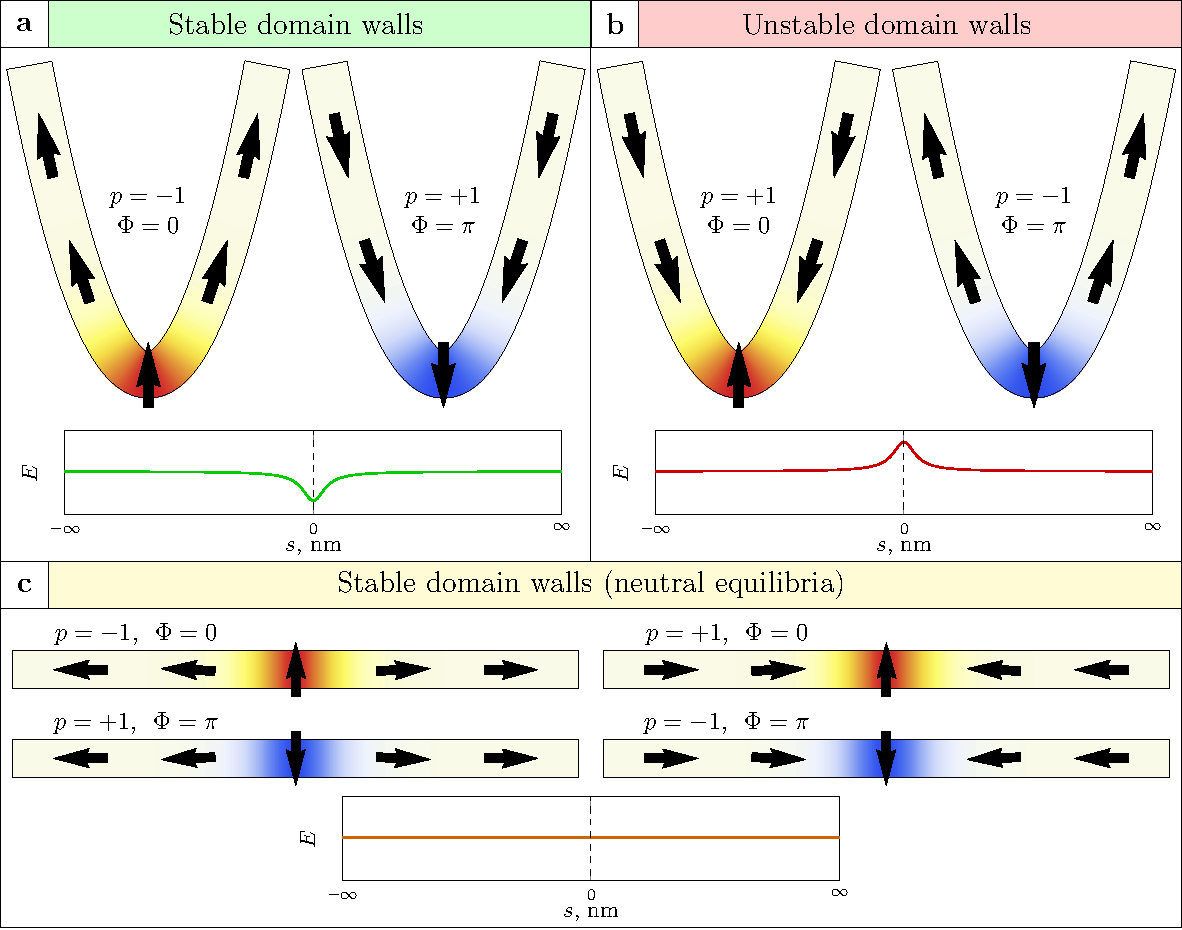
\includegraphics[width=0.9\linewidth]{fig_parabola_n_straight_stripe}}
	\caption{\textbf{Curvature-induced asymmetrical stability of transversal DWs and their comparison with similar DWs in straight stripes.} \textbf{(a)},~Stable tail-to-tail and head-to-head DWs and their energy landscape on DWs position along the parabolic stripe. The energy landscape is calculated by means of the $q$ -- $\Phi$ model. The potential well at the apex region appears due to the influence of the curvature-induced DMI. \textbf{(b)},~Unstable head-to-head and tail-to-tail transversal DWs in a parabolic stripe and corresponding to them potential wall. \textbf{(c)},~Transversal DWs in a straight stripe, with their neutral stability within the framework of the $q$ -- $\Phi$ model. Adapted with permission from~\cite{Volkov19c}.}
	\label{fig:Parabola_n_straight_DWs}
\end{figure}
%==================================================================/

The energy~\eqref{eq:dw_total_energy_angular} for DW reads
\begin{equation}\label{eq:dw_energy}
\frac{\mathcal{E}^\textsc{dw}}{2}\approx\frac{1}{\Delta}+\Delta\,\left(1+\varepsilon\sin^2\varPhi\right)+p\pi\varkappa(q)\cos\varPhi+\mathcal{O}\left(\varkappa^2\right),
\end{equation}
where the condition $\varkappa\Delta\ll1$ was applied when integrating. The first and second terms represent the competition between the isotropic exchange and anisotropy terms, and defines the DW width in rectilinear system. While the last term determines the curvature-induced DMI contribution.

Firstly, lest us consider the systems with localized curvature $\varkappa(\pm\infty)=0$, i.e. \textit{parabola}-shaped system. Minimization of~\eqref{eq:dw_energy} with respect to $q$ and $\varPhi$ results in the following equilibrium values
\begin{equation}\label{eq:dw_eq_state}
\varkappa'\left(q_0\right)=0,\quad\cos\varPhi_0=-p.
\end{equation}
Thus the DW is pinned at the maximum of the curvature, and the phase selectivity takes place: the head-to-head DW is directed outward while the tail-to-tail one is directed inward the bend; see Fig.~\ref{fig:Parabola_n_straight_DWs}(a). There is an intuitive explanation: the choice of $\varPhi_0$ defined by~\eqref{eq:dw_eq_state} makes the magnetization distribution more homogeneous, see
Figs.~\ref{fig:Parabola_n_straight_DWs}(a) and~\ref{fig:Parabola_n_straight_DWs}(b), which decreases the exchange energy.

The exchange-driven effective DMI leads to the reshaping of the DW total energy \eqref{eq:dw_energy} in a way of appearance additional potentials corresponding to the type of DWs: (i) In the case of two transversal DWs with $p=+1$, $\varPhi=\pi$ and with $p=-1$, $\varPhi=0$ the curvature-induced DMI form a potential well at the apex region, see Fig.~\ref{fig:Parabola_n_straight_DWs}(a). (ii) In the case of two other possible configuration of transversal DWs with $p=+1$, $\varPhi=0$ and with $p=-1$, $\varPhi=\pi$, there is a potential wall, see Fig.~\ref{fig:Parabola_n_straight_DWs}(b).  This is in contrast to a straight stripe system, where all four possible types of transversal DWs are energetically equal and stable in a sense of neutral equilibria in the $q-\varPhi$ model framework, see Fig.~\ref{fig:Parabola_n_straight_DWs}(c).

As it follows from~\eqref{eq:dw_energy}, the equilibrium value of the domain wall width $\Delta_0 = 1$ is the same as for a straight wire. However, if the wall is not in the equilibrium position and the collective variables $(q,\varPhi)$ deviate from the equilibrium \eqref{eq:dw_eq_state}, the DW width is modified. This problem will be discussed in the next section.

\subsection{Dynamics of the domain wall.}

The dynamics of magnetization is governed by the phenomenological LLG equation~\eqref{eq:llg}. In terms of $\{q,\varPhi,\Delta\}$ it reads~\cite{Yershov15b,Yershov18a}
\begin{equation}\label{eq:dw_qPhi_motion}
\begin{split}
\frac{\alpha_\textsc{g}}{\Delta}\dot{q}+p\dot{\varPhi} = &-p\pi\frac{\partial\varkappa(q)}{\partial q}\cos\varPhi,\\
p\dot{q}-\alpha_\textsc{g}\Delta\dot{\varPhi} = &-p\pi\varkappa(q)\sin\varPhi+\varepsilon\Delta\sin 2\varPhi.
\end{split}
\end{equation}
The dynamics of the DW width can be described as $\alpha_\textsc{g}\pi^2\dot{\Delta}/12=1/\Delta-\Delta\left(1+\varepsilon\sin^2\varPhi\right)$, which shows that $\Delta$ relaxes towards its equilibrium value $\Delta_0=1/\sqrt{1+\varepsilon\sin^2\varPhi}$. The characteristic time of this relaxation is proportional to the damping $\propto \alpha_\textsc{g}$~\cite{Hillebrands06}. Usually $\alpha_\textsc{g}\ll1$, therefore one can conclude that the DW width is a slave variable $\Delta(t) = \Delta[\varPhi(t)]$ and DW dynamics can be described by the set~\eqref{eq:dw_qPhi_motion}  with the equilibrium DW width $\Delta=\Delta_0$. From \eqref{eq:dw_qPhi_motion} it follows that the gradient of the curvature is a driving force for DWs. The physical origin of this force is the curvature-induced DMI driven by the exchange.

%==================================================================\
\begin{figure}[t]
	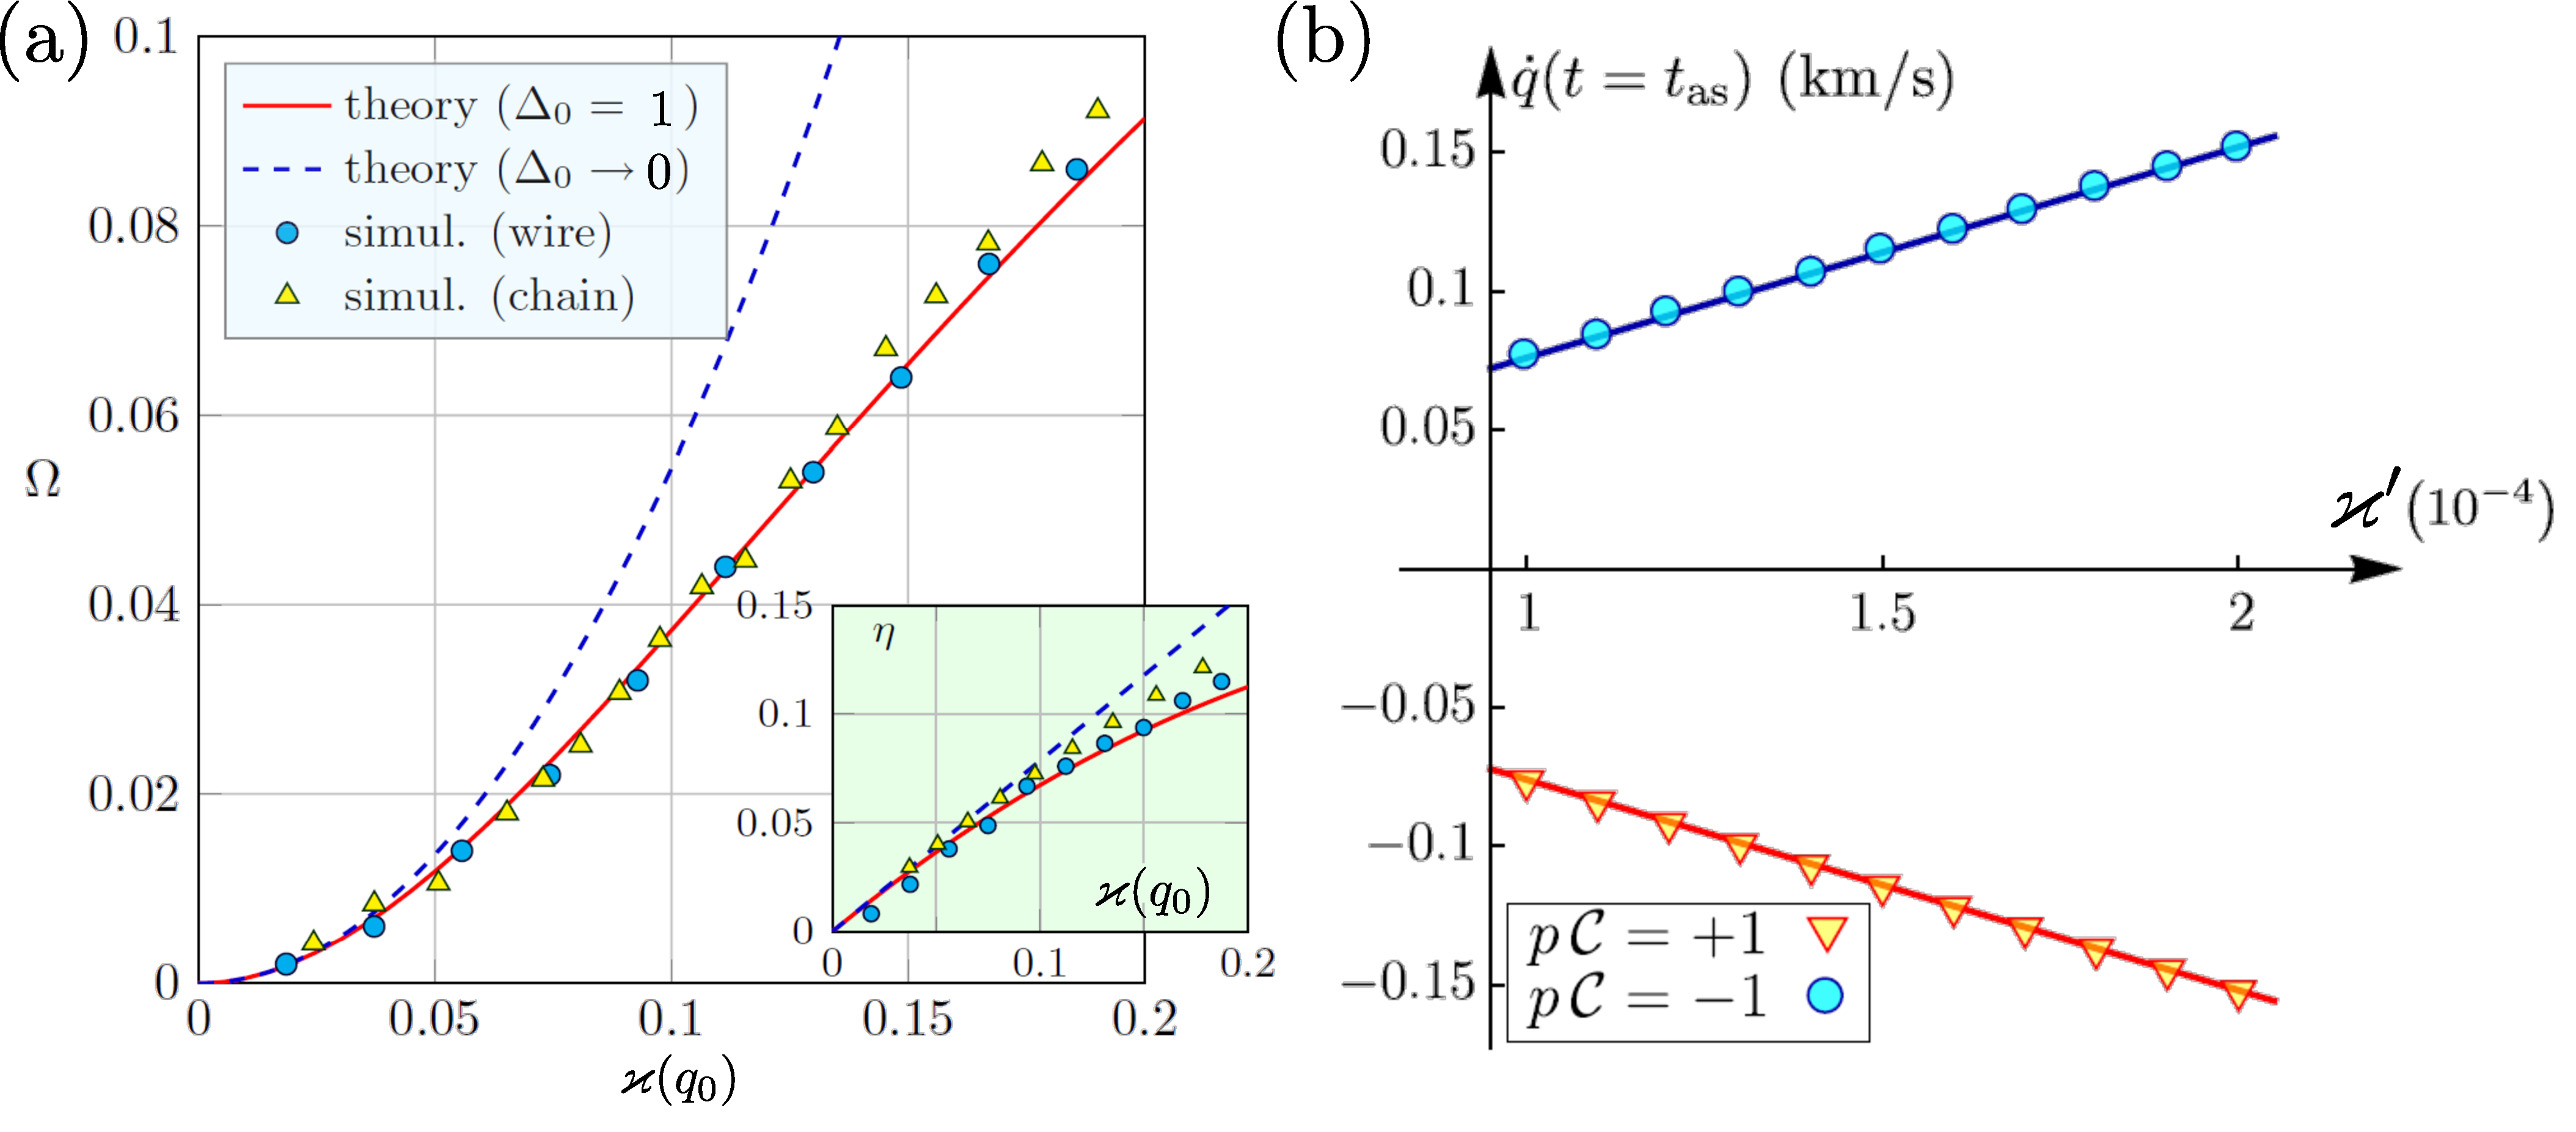
\includegraphics[width=\textwidth]{fig_dw_dynamics_curved}
	\caption{\label{fig:dw_wire_2}%
		\textbf{DW dynamics in curved wires.} (a) DW velocity $\dot{q}$ as a function of the gradient of the curvature in the Euler spiral. (b) Eigenfrequency of the DW oscillations in vicinity of the equilibrium -- the extreme point of parabolic wire bend.  In (a) and (b) lines correspond to the analytical predictions and symbols to the results of micromagnetic simulations. Panel (a) is reproduced from~\cite{Yershov18a}; panel (b) is reproduced from~\cite{Yershov15b}.}
\end{figure}
%==================================================================/

{\it Curvature-induced motion of domain wall.} For the wires with monotonic increasing/decreasing curvature as a function of the arc length the curvature gradient in Eqs.~\eqref{eq:dw_qPhi_motion} results in a driving force, i.e. DW can be moved without any external driving~(field or current) and pinning. In the limit case of \textit{Euler spiral}, see Fig.~\ref{fig:Geometries_n_curvatures}(e), the DW can move with constant velocity
\begin{equation}\label{eq:velocity_euler_spiral}
\mathscr{V}=-p\,\mathcal{C}\,\frac{\varkappa'}{\alpha_\textsc{g}},\quad\cos\varPhi_0=\mathcal{C}=\pm1.
\end{equation}
The phase during the dynamics behaves as $\varPhi\approx\varPhi_0+p/\left(\alpha_\textsc{g} \mathscr{V} \overline{t}\right)$, which in long time approximation results in $\varPhi\left(\overline{t}\to\infty\right)=\varPhi_0$. Hence, the parameter $\mathcal{C}$ is interpreted as the DW magnetochirality~\cite{Kim14}.  The corresponding geometry-induced DW velocity for the Euler spiral reaches up to 150 m/s, see Fig.~\ref{fig:dw_wire_2}(a). For the case of curved wires~\cite{Lewis09,Nahrwold09,Wartelle18} with curvature in the range $\kappa\in\left[0;1/150\right]$ nm$^{-1}$ the corresponding curvature-induced DW velocity is expected to be about 80 m/s.

The direction of the geometry-induced DW motion\footnote{One has to notice a one-to-one correspondence between natural	parameter $\xi$ and gradient of the curvature $\varkappa'$ with DW magnitochirality $\mathcal{C}$: change of the natural parameter sign results in the changing of gradient of the curvature and DW magnitochirality	signs, therefore direction of DW motion physically is the same.} is determined by the product of the DW magnetochirality, topological charge, and gradient of the curvature $\mathscr{V}\propto p\,\mathcal{C}\varkappa'$, see Fig.~\ref{fig:dw_wire_2}(a). The geometry-induced dynamics are accompanied by the DW motion in the area of bigger curvature. In this way, in the energy~\eqref{eq:dw_energy} the geometry-induced DMI term becomes dominant. This term fixes the DW phase $\cos\varPhi=\pm1$, which depends on the sign of the product of the topological charge $p$ and curvature $\varkappa$, see Eq.~\eqref{eq:dw_energy}. Therefore, the transition to the precessional regime becomes suppressed. This effect can be interpreted as the curvature-induced suppression of the Walker limit~\cite{Yershov18a}. This is in contrast to the case of field-driven DWs in a straight wire, where the phase of the DW is not fixed (Zeeman term in the energy of DW is independent of the phase~\cite{Malozemoff79,Hillebrands06}).

The DW velocity~\eqref{eq:velocity_euler_spiral} is similar to the well-known expression $\mathscr{V}_u = u \beta/\alpha_\textsc{g}$ in magnetic stripes with biaxial anisotropy caused by the Zhang--Li mechanism~\cite{Bazaliy98,Zhang04}, where $\beta$ is a nonadiabatic spin-transfer parameter. Current-induced translational DW motion takes place only if $u<u_\textsc{w}$, where $u_\textsc{w}$ is Walker current~\cite{Thiaville05}. However, for the case of a geometry-induced motion, a Walker-limit-like effect of the transition to the precessional regime does not appear and the DW demonstrates a high-speed translational motion without any external driving. However, for the current-induced dynamics of DW in an uniaxial~($\varepsilon=0$) circular-shaped wires~($\varkappa=\text{const}$) curvature results in the appearance of Walker limit~\cite{Yershov16}
\begin{equation}
u_\textsc{w}^\varkappa=\frac{\alpha_\textsc{g}}{|\alpha_\textsc{g}-\beta|}\pi\varkappa.
\end{equation}

One can see that DW velocity is increasing with decreasing Gilbert damping~$\alpha_\textsc{g}$, see Eq.~\eqref{eq:velocity_euler_spiral}. For the limit case of vanishing damping~($\alpha_\textsc{g}\to0$) the velocity of the DW increases exponentially with time, and its transverse magnetization component orients perpendicular to the wires plane with $\varPhi(\alpha_\textsc{g}=0)\to-\mathcal{C}\pi/2$.

%Geometry-induced motion of DWs desctibed by Eqs.~\eqref{eq:dw_qPhi_motion} can be compared with so called automotion of DW in curved systems~\cite{Chauleau10,Richter16,Mawass17}. This type of motion can be realized relying on: (i) The transformation of DWs from transverse to vortex types after the action of current pulse~\cite{Chauleau10}, see Figs.~\ref{fig:automotion}(a)-\ref{fig:automotion}(f). In this case, the motion of DW is caused by the modification DW phase $\Phi$~(a canonically conjugated variable to DW position $q$). Such type of motion is possible for the duration of excitation is short compared to the relaxation time of the DW structure~\cite{Chauleau10}. (ii) The second mechanism is relying on the motion of DWs in systems with coordinate-dependent cross sectional area of a nanostripe~\cite{Richter16,Mawass17}, see Fig.~\ref{fig:automotion}(g). In this case, the motion of DW is caused by the minimization of DW energy in the narrow area of asymmetric ring~\cite{Mawass17}. One should note that with increasing the gradient of ring's aspect ratio the velocity of DW increases.

Geometry-induced motion of DWs desctibed by Eqs.~\eqref{eq:dw_qPhi_motion} can be compared with so called automotion of DW in curved systems~\cite{Chauleau10,Richter16,Mawass17}. This type of motion can be realized relying on: (i) The transformation of DWs from transverse to vortex types after the action of current pulse~\cite{Chauleau10}. In this case, the motion of DW is caused by the modification DW phase $\Phi$~(a canonically conjugated variable to DW position $q$). Such type of motion is possible for the duration of excitation is short compared to the relaxation time of the DW structure~\cite{Chauleau10}. (ii) The second mechanism is relying on the motion of DWs in systems with coordinate-dependent cross sectional area of a nanostripe~\cite{Richter16,Mawass17}. In this case, the motion of DW is caused by the minimization of DW energy in the narrow area of asymmetric ring~\cite{Mawass17}. One should note that with increasing the gradient of ring's aspect ratio the velocity of DW increases.

%==================================================================\
%\begin{figure}[t]
%	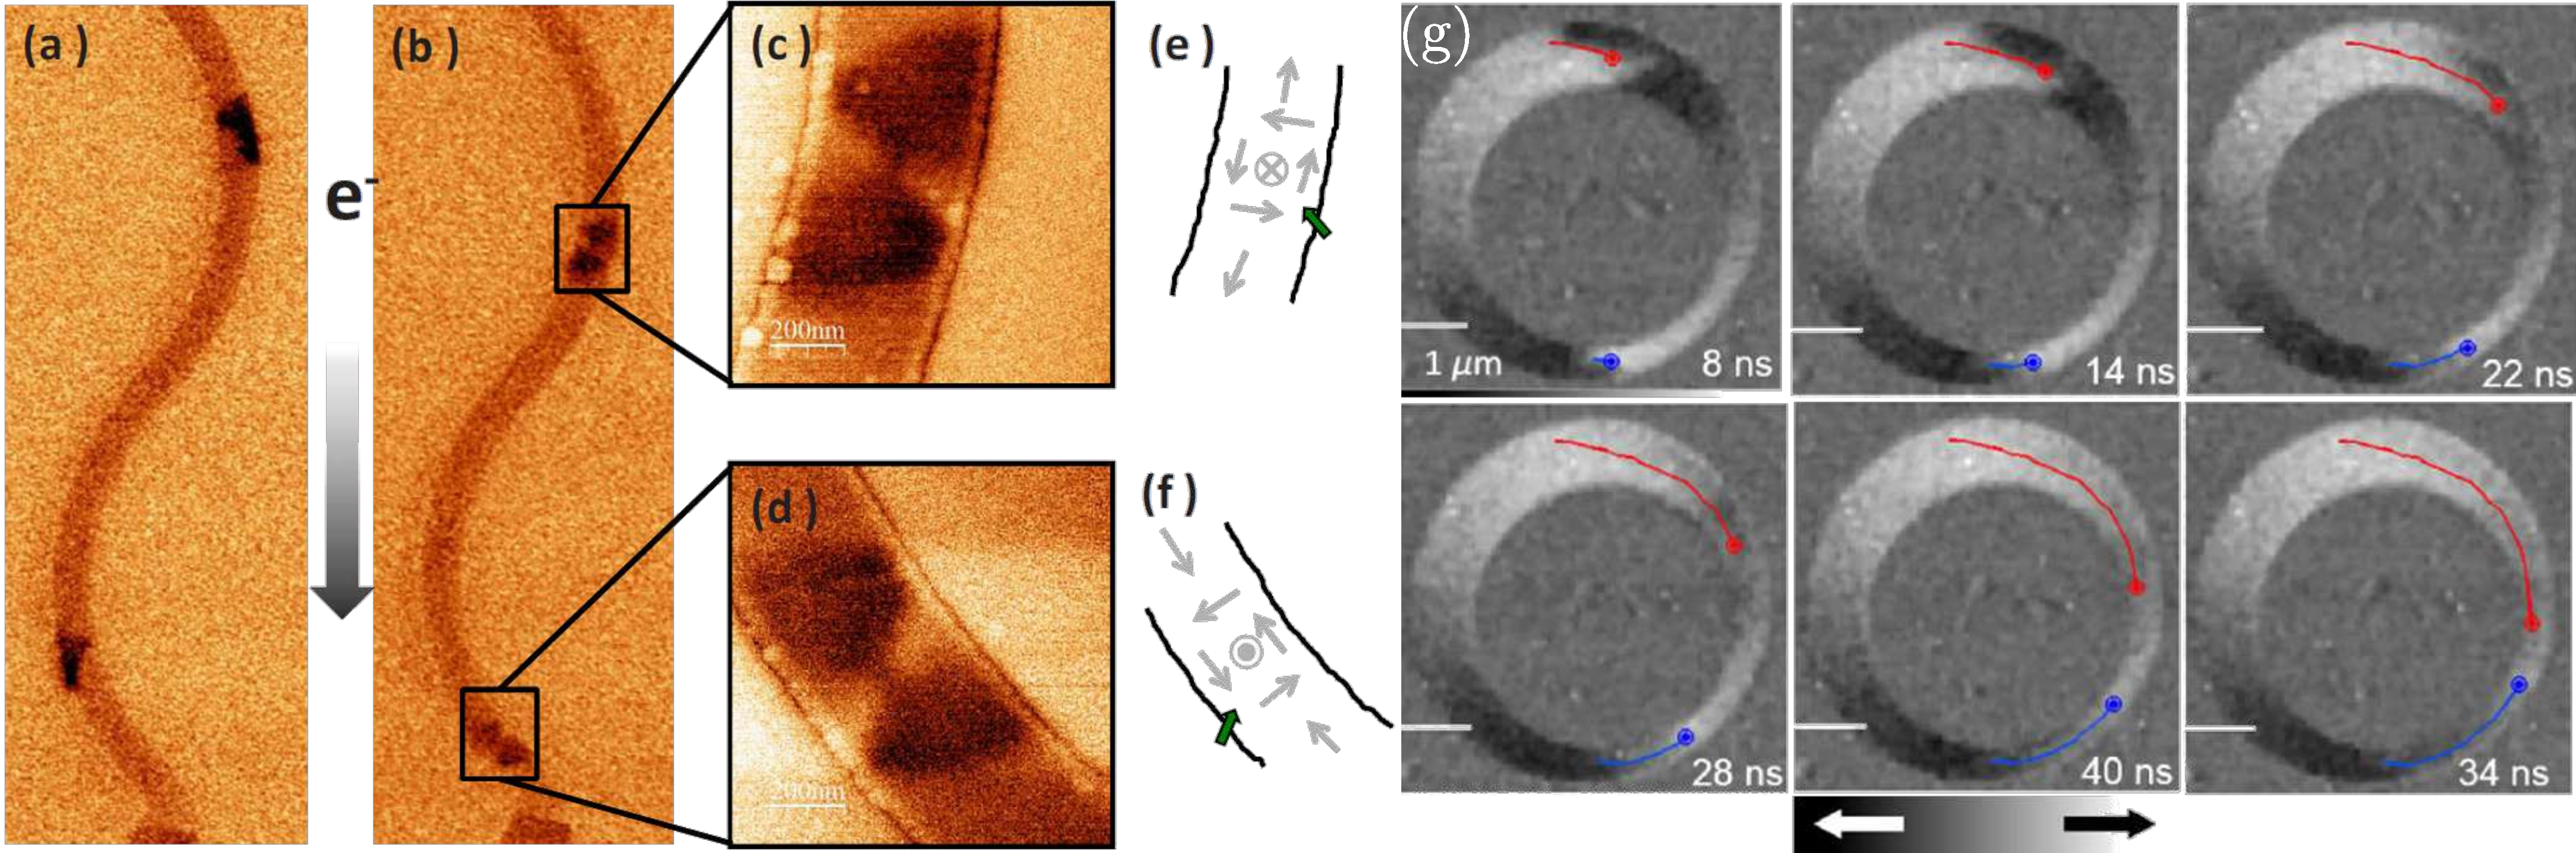
\includegraphics[width=\textwidth]{fig_automotion}
%	\caption{\label{fig:automotion}%
%		\textbf{Automotion of DWs.} (a)-(b) Magnetic force microscopy images of the initial and final magnetic states of the entire S-shaped nanostrip showing two transverse and two vortex DWs, respectivelly . In (b) two vortex DWs displaced by 1.5 and 1.7 $\mu$m after transforming under a 1 ns current pulse of 3.6 TA/m$^2$ amplitude. (c) and (d) zoom on the vortex DWs, with schematics shown in (e) and (f). (g) Time-resolved STXM XMCD snapshots of automotive DWs motion during the switching process from the onion to the vortex state in the ferromagnetic ring. Red and blue lines in (g) illustrate the averaged trajectory of the vortex DWs. Panels (a)-(f) are reproduced from~\cite{Chauleau10}; panel (g) is reproduced from~\cite{Mawass17}.}
%\end{figure}
%==================================================================/

{\it Curvature-induced pinning of the domain wall.} The equations of motion~\eqref{eq:dw_qPhi_motion} can be linearized with respect of small deviations of DW position $\tilde{q}=q-q_0$ and phase $\tilde{\phi}=\varPhi-\varPhi_0$ in the vicinity of equilibrium position~\eqref{eq:dw_eq_state}. For the limit case of small curvature $\varkappa\ll1$ and $\varepsilon=0$ the equations of motion~\eqref{eq:dw_qPhi_motion} linearized with respect to the deviations reads~\cite{Yershov15b}
\begin{equation}\label{eq:dw_qPhi_motion_linear}
\left(1+\alpha_\textsc{g}^2\right)\left\|\begin{matrix}
\dot{\tilde{q}}\\
\dot{\tilde{\phi}}
\end{matrix}\right\|=\pi\left\|\begin{matrix}
0 & \varkappa(q_0)\\
\varkappa''(q_0)&-\alpha_\textsc{g}\varkappa(q_0)
\end{matrix}\right\|\cdot\left\|\begin{matrix}
\tilde{q}\\
\tilde{\phi}
\end{matrix}\right\|.
\end{equation}
For the case of small damping the solution of~\eqref{eq:dw_qPhi_motion_linear} results in harmonic decaying oscillations with frequency $\Omega$ and modified effective friction $\eta$ defined as
\begin{equation}
\Omega \approx \pi\sqrt{|\varkappa(q_0)\varkappa''(q_0)|},\quad \eta\approx \alpha_\textsc{g}\frac{\pi}{2}\varkappa(q_0).
\end{equation}
Eigenfrequency of the DW oscillations in vicinity of the equilibrium position is presented in Fig.~\ref{fig:dw_wire_2}(b). As it was mentioned above, the circular geometry does not generate any pinning potential, therefore the eigenfrequency of the DW oscillations in such geometry is $\Omega=0$. The value of pinning potential increases with the increasing of the curvature, see Fig.~\ref{fig:dw_wire_2}(b), which results in the increasing of the deppining field up to 10-20 mT~\cite{Volkov19c,Lewis09}.

\subsection{Domain wall depinning experiments} \label{subsubsec:Parabola_experiments}

%==================================================================\
\begin{figure}[b]
	\center{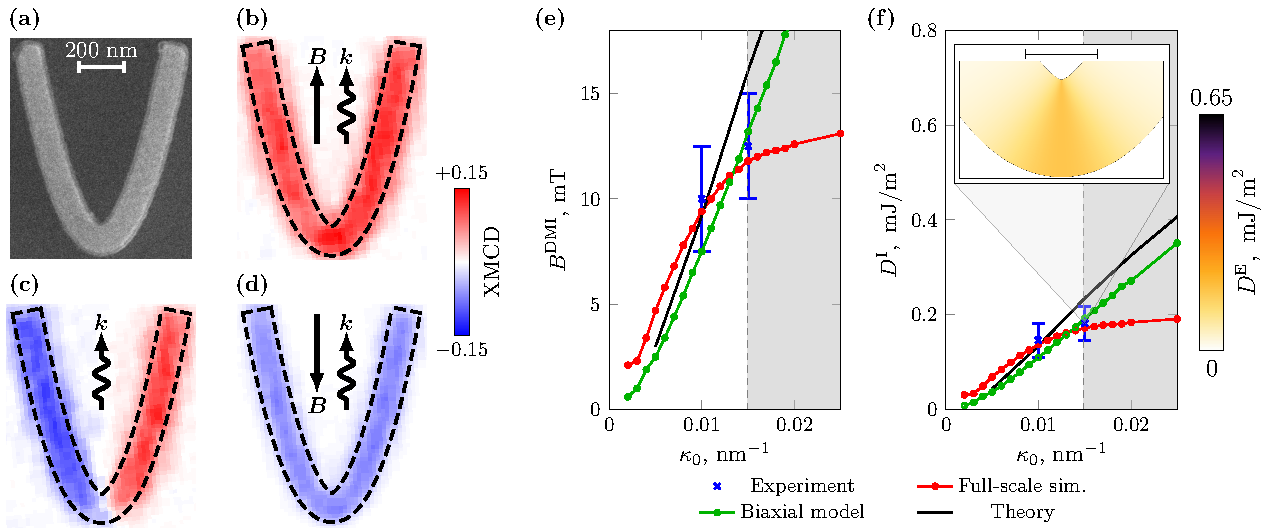
\includegraphics[width=1.0\linewidth]{fig_domain_wall_experiment}}
	\caption{\textbf{Field-induced state change in parabolic nanostripes.} \textbf{(a)}, Scanning electron microscopy image of a patterned stripe with $L=2$~$\mu$m length, $W=135$~nm width, and $\kappa_0=0.015$~nm$^{-1}$ vertex curvature. The main magnetic states imaged by XMCD-PEEM appearing during the field reversal are \textbf{(b)}, tail-to-tail domain wall, \textbf{(c)}, homogeneous magnetic distribution along the parabola, and \textbf{(d)}, head-to-head domain wall. \textbf{(e)}, The dependence of the domain wall depinning field on the vertex curvature. \textbf{(f)}, The dependence of curvature-driven extrinsic DMI constant on the vertex curvature. Adapted with permission from~\cite{Volkov19c}.}
	\label{fig:Experiment_parabola}
\end{figure}
%==================================================================/

Although the curvilinear exchange-driven chiral effects are generic, they are difficult to be found in experiments because they are shaded by other effects or interactions such as the long range magnetostatic interaction. However, the exchange interaction alone in a curved system will not lead to curvature-induced chiral effects. A further requirement is the existence of an anisotropy, which reflects the shape of the curvature. Thus, recently it was experimentally explored the appearance of curvature-induced chiral responses in a flat parabolic stripes made from a soft ferromagnetic material (Permalloy)~\cite{Volkov19c}, see Fig.~\ref{fig:Experiment_parabola}(a). Such system contains a shape-induced anisotropy, which reflects the parabolic shape due the magnetostatic or dipole-dipole interaction. It was predicted theoretically that the magnetization reversal of flat parabolic stripes shows a two-step process: (i) The first switching event occurs due to the expelling of a transversal tail-to-tail DW from a pinning potential induced by the exchange-driven DMI. This process corresponds to the transition from a red contrast of x-ray magnetic circular dichroism photoelectron emission microscopy (XMCD-PEEM), see Fig.~\ref{fig:Experiment_parabola}(b), to a dipolar one with blue-red contrast, see Fig.~\ref{fig:Experiment_parabola}(c). (ii) The second switching event corresponds to the nucleation of a head-to-head DW from the end of a parabolic branch and its propagation into the apex area, which leads to the appearance of blue XMCD-PEEM contrast, see Fig.~\ref{fig:Experiment_parabola}(d). Experimental investigations of static magnetization states appearing during hysteresis loops confirmed the predicted switching mechanism. Supporting these experimental results with micromagnetic simulations and analytical calculations it became possible to quantify the strength of the effective exchange-driven DMI constant $D^\mathrm{E}$ from the first switching field $B^\textrm{DMI}$~\cite{Volkov19c}, see Fig.~\ref{fig:Experiment_parabola}(e): 
\begin{equation} \label{eq:experimental_DMI_coef}
D^\textrm{E} = B^\textrm{DMI} \, M_s \, \sqrt{\frac{A}{K}} \, \sqrt{\dfrac{2 \, \pi \, W}{H \, \left[ 2 \ln(W/H)+3 \right]}},
\end{equation}   
where $\ell$ is the exchange length, with $W$ and $H$ being stripe width and thickness, respectively. It was found to be remarkably strong compared to the surface-induced DMI and also its value could be tuned by tailoring the local curvature and shape of ferromagnets, see Fig.~\ref{fig:Experiment_parabola}(f). The exchange-driven DMI constant determined experimentally~\cite{Volkov19c} is relatively strong and comparable with reported values obtained for asymmetric Co sandwiches~\cite{Boulle16}.
